\section*{Autres informations}
\label{sec:autres}
\addcontentsline{toc}{section}{Autres informations}

\subsection*{Liens utiles}
\label{subsec:liens}
\addcontentsline{toc}{subsection}{Liens utiles}
Pour ceux qui sont intéressés par le domaine de la finance ou qui cherchent à étendre leurs champs d'expertise, la désignation professionnelle CFA peut être une très bonne option. C'est sans doute la désignation du monde de la finance qui est la plus reconnue à l'international et un nombre considérable d'actuaires la possèdent. Afin d'obtenir cette désignation, l'on doit passer trois examens (\emph{Level I, II} et \emph{Level III}) et avoir quatre ans d'expérience pertinente dans le milieu de la finance. Concernant l'expérience demandée, il est difficile de connaître les critères exactes du CFA Institute mais, généralement, il faut qu'une majorité du temps de travail de ces quatre années soit relié à la gestion d'actifs au sens large. Les examens \emph{Level II \emph{et} Level III} sont offerts seulement une fois par année, le premier samedi du mois de juin, alors que le \emph{Level I} est également offert au mois de décembre. Pour plus d'informations, consulter la page du \href{https://www.cfainstitute.org/Pages/index.aspx}{\emph{CFA Institute}}. Vous pouvez également lire l'article \href{http://blog.coachingactuaries.com/why-would-actuaries-consider-getting-a-cfa/}{\emph{Why would Actuaries consider getting a CFA?}}.\vspace{\baselineskip}

Ceux qui sont intéressés par l'informatique et le \emph{data science} pourront s'informer au sujet de la création du \href{http://www.casact.org/press/index.cfm?fa=viewArticle&articleID=3083}{CAS Institute}.\vspace{\baselineskip} 

\newpage
\subsection*{Changements aux prérequis pour devenir Associé}
\label{subsec:changeasa}
\addcontentsline{toc}{subsection}{Changements aux prérequis pour devenir Associé}
\subsubsection*{SOA}
La SOA est présentement en processus de restructuration des prérequis pour devenir Associé. Ils ont fait une annonce officielle à la fin du mois de juin pour préciser davantage la nouvelle structure, qui devrait être effective à partir du $1^{ier}$ juillet 2018. Le plus gros changement est l’ajout de deux nouveaux examens, mais ce sont toutes les composantes qui vont être modifiées.\vspace{\baselineskip} 

\textbf{Voici les éléments clés de l’annonce de juin :}
\begin{itemize}
\item Ajout de la tarification et des méthodes de réserve à l’examen C/4
\item Tous les concepts liés aux produits dérivés seront désormais dans l'examen MFE/3F (à l'exception des swaps de taux d'intérêt)
\item Retrait des concepts plus avancés de l’examen MFE/3F (processus stochastiques, mouvement brownien, modèles de taux d’intérêt, etc.)
\item Ajout d’un examen sur les statistiques appliquées – \emph{Statistics for Risk Modeling}  
\item Ajout d’un examen sur l’analyse de données - \emph{Predictive Analytics}
\item Le VEE finance comptera une partie sur la comptabilité 
\end{itemize}
\vspace{\baselineskip} 

\subsubsection*{CAS}
La CAS a déjà annoncé qu’elle reconnaîtrait le nouveau format des examens FM/2, MFE/3F (IMF) et C/4 (STAM/MAS-2) à partir de l’été 2017. 

\textbf{Voici les éléments clés de l’annonce de juin :}
\begin{itemize}
\item Modification de l'examen S (MAS-1) 
\end{itemize}
\vspace{\baselineskip} 

Quelques liens supplémentaires :
\begin{enumerate}
\item \href{https://www.soa.org/Education/General-Info/2016-asa-cera-curriculum-changes.aspx}{Annonce du 28 juin par la SOA}
\item \href{https://soa.qualtrics.com/CP/File.php?F=F_0TDd9bj143TrCW9}{Annonce préliminaire de la SOA (janvier 2016)}
\item \href{https://www.soa.org/Education/General-Info/2016-transition-rules-asa-candidated.aspx}{L’équivalence des examens actuels dans le système à venir}
\item \href{http://www.casact.org/press/index.cfm?fa=viewArticle&articleID=3273}{Annonce de la CAS pour le nouveau format de FM/2 et MFE/3F}
\end{enumerate}

\begin{figure}[hp]
\begin{center}
\textbf{Changements aux prérequis pour devenir Associé (SOA)}\par\medskip
\end{center}
\hfill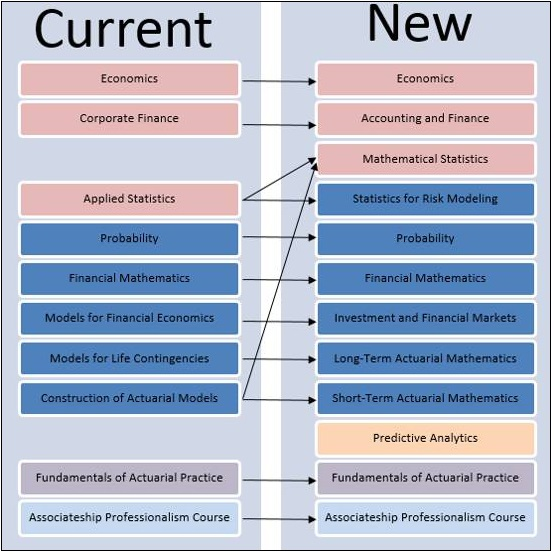
\includegraphics[scale=0.8]{Change_ASA.PNG}\hspace*{\fill}
\caption{Équivalences des examens actuels dans le système à venir (SOA)}
\end{figure}
\par
\begin{figure}[hp]
\begin{center}
\textbf{Changements aux prérequis pour devenir Associé (CAS)}\par\medskip
\end{center}
\hfill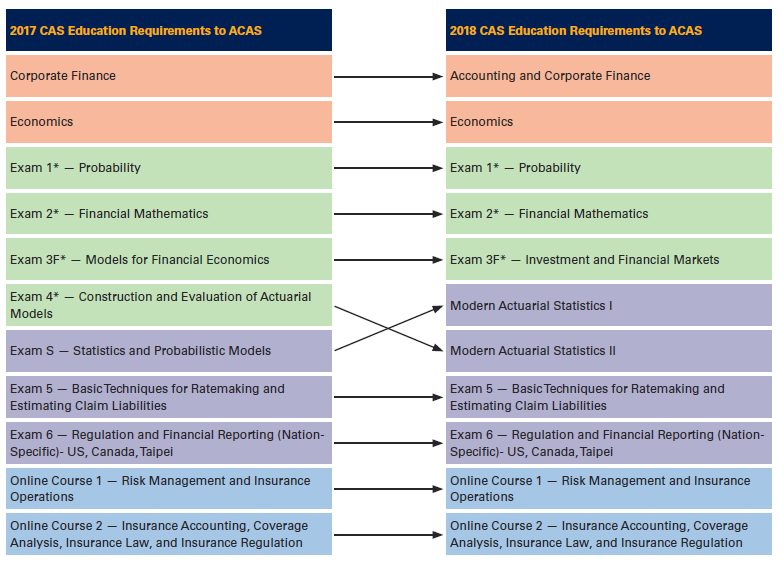
\includegraphics[scale=0.6]{Change_ASA_CAS.PNG}\hspace*{\fill}
\caption{Équivalences des examens actuels dans le système à venir (CAS)}
\end{figure}
\par

\newpage